%%%%%%%%%%%%%%%%
\section{Introduction}

\begin{frame}{Introduction}{}
    \begin{figure}[H]
        \centering
        \includegraphics[width=.6\linewidth]{figures/frontpage}
    \end{figure}
    \begin{itemize}
         \item What is an Autonomous Surface Vessel (ASV)
         \item Bathymetric Measurements
         \item Control of an ASV
    \end{itemize}
\end{frame}

\begin{frame}{Introduction}{Use Case}
    \begin{figure}[H]
        \centering
        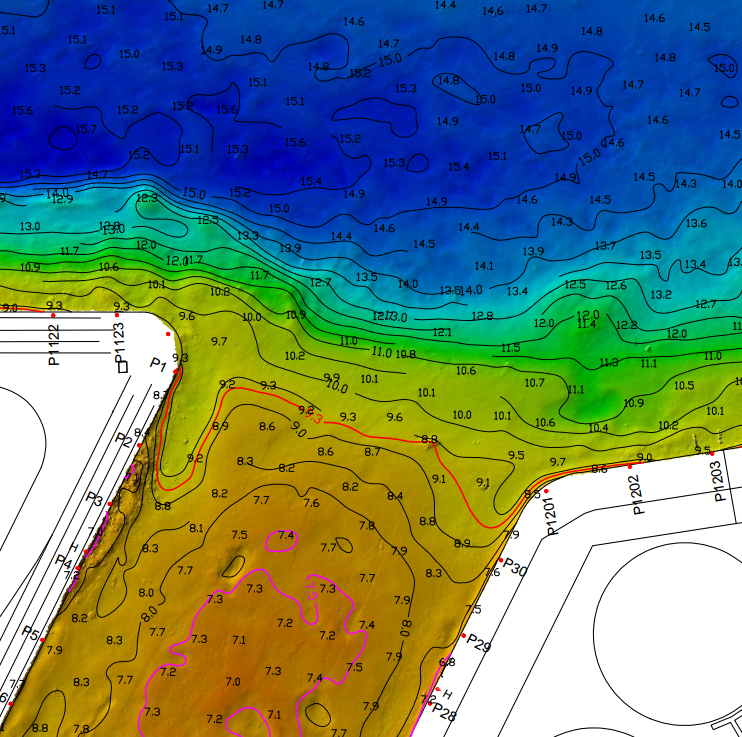
\includegraphics[width=.4\linewidth]{figures/smallDebthMapAalborg}
    \end{figure}
    \begin{itemize}
        \item Used by Port of Aalborg 
        \item Problem: No recent knowledge of depths of the port
        \item Solution: Automate smaller unmanned vessel
    \end{itemize}
\end{frame}

\begin{frame}{Introduction}{Functional Requirements}
    \begin{itemize}
        \item[\textbf{A:}] It shall be possible to select the area in which the bathymetric measurements are to be performed.
        \item[\textbf{B:}] The ASV shall be able to plan a route, such that the entire survey area is mapped.
        \item[\textbf{C:}] The ASV shall be able to follow the planned route.
        \item[\textbf{D:}] The controller shall be robust to external disturbances.
        \item[\textbf{E:}] The THU shall not exceed 30 cm with a 95\% confidence interval.
        \item[\textbf{F:}] The ASV shall record and store data locally for extraction at the end of the survey.
        \item[\textbf{G:}] It shall be possible to give the ASV a command to stop and steer it back to land.
    \end{itemize}
\end{frame}

\section{System Description}
\begin{frame}{System Description}{}
    \begin{minipage}{0.45\linewidth}
    \begin{figure}[H]
        \centering
        \includegraphics[width=1\linewidth]{figures/system}
    \end{figure}        
    \end{minipage}\hfill      
    \begin{minipage}{0.45\linewidth}
    \begin{figure}[H]
        \centering
        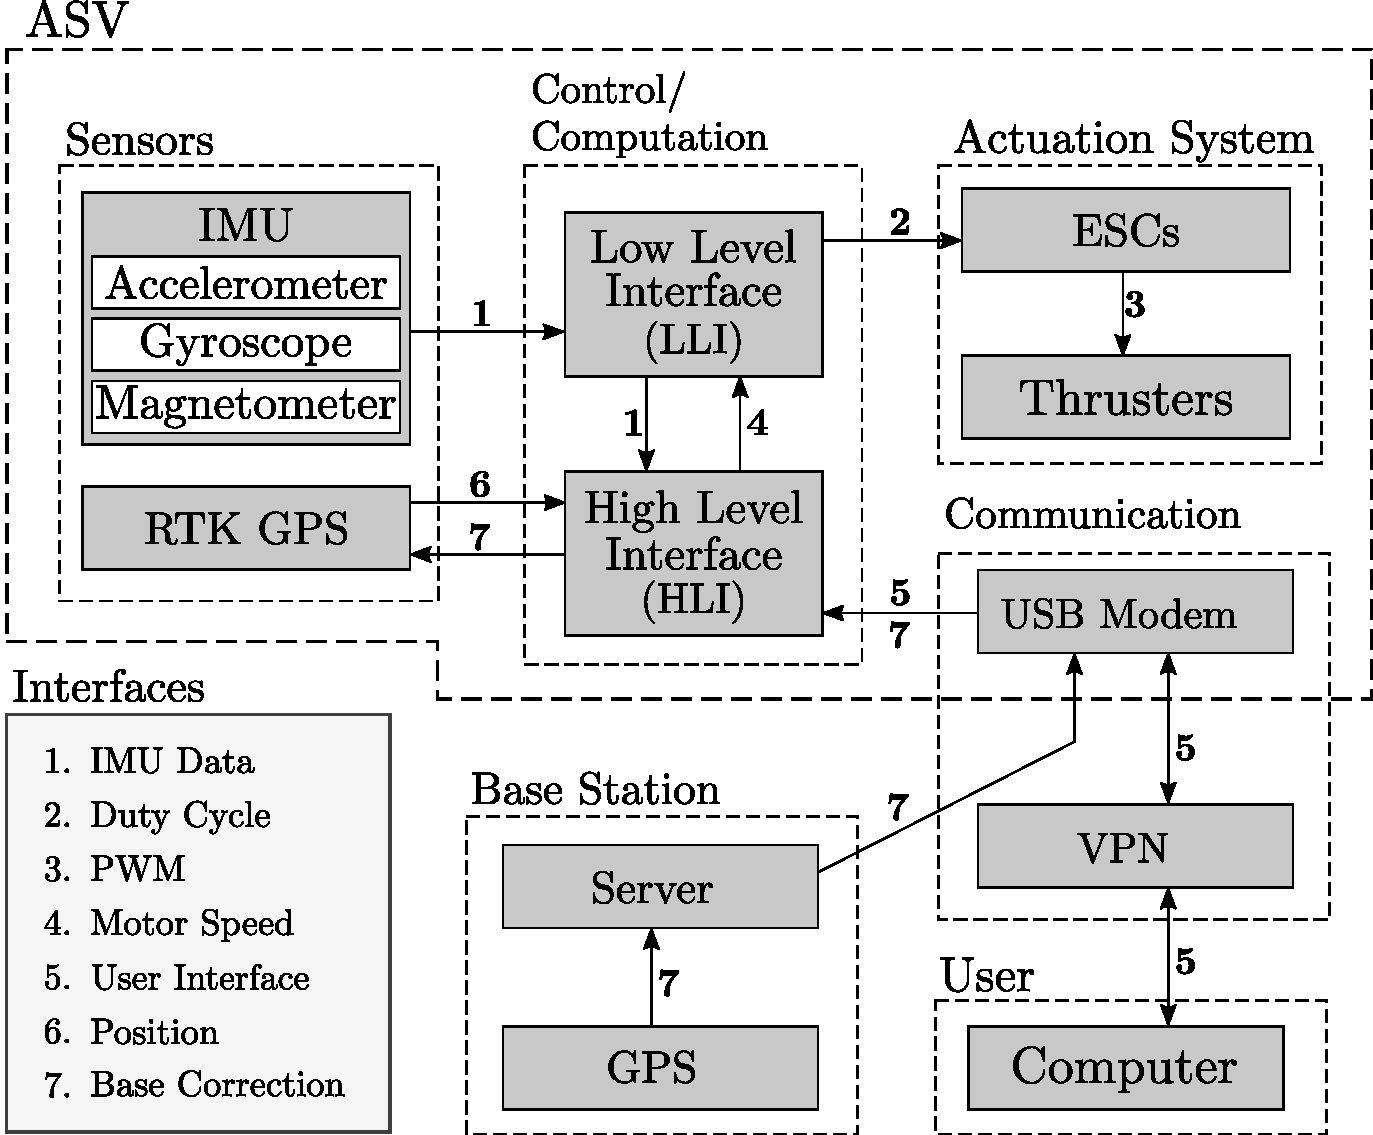
\includegraphics[width=1\linewidth]{figures/systemDiagram5}
    \end{figure}                
    \end{minipage}\hfill \\
\end{frame}

\begin{frame}{System Description}{RTK GPS}
    \begin{figure}[H]
        \centering
        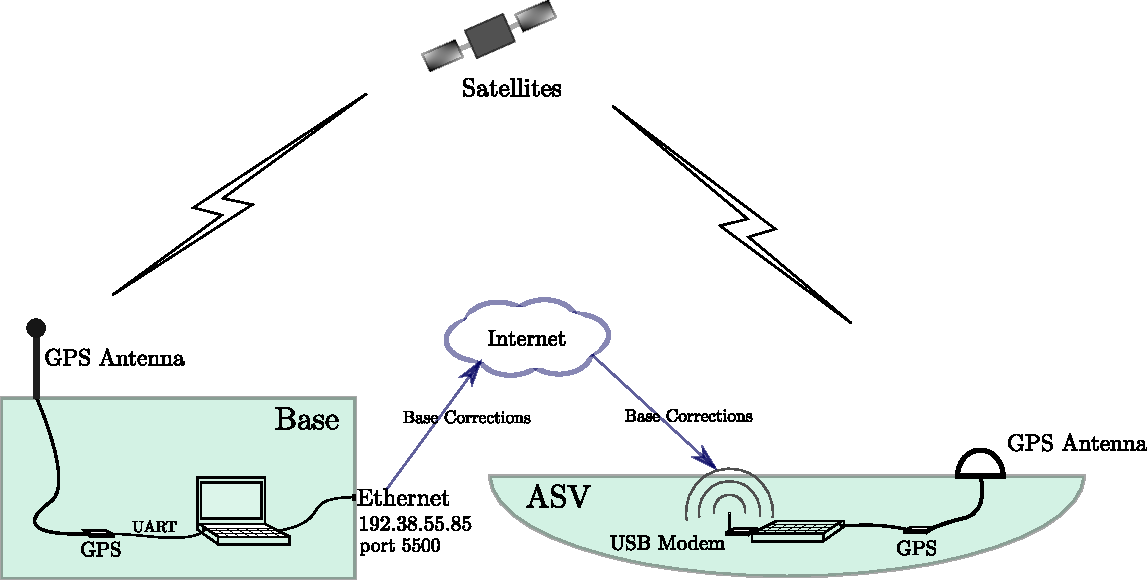
\includegraphics[width=0.7\linewidth]{figures/comunicationSetup}
    \end{figure}        

\end{frame}

%%%%%%%%%%%%%%%%
\section{Model}

%\subsection{Reference Frames}
\begin{frame}{Model}{Reference Frames}
    \begin{minipage}{0.65\linewidth}
        \begin{figure}[H]
            \centering
            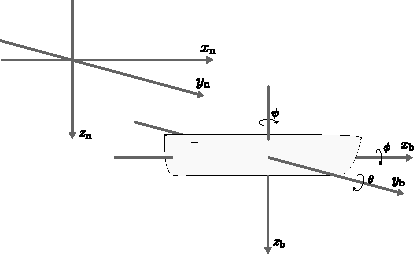
\includegraphics[width=1\linewidth]{figures/boat3D}
        \end{figure}        
    \end{minipage}\hfill      
    \begin{minipage}{0.3\linewidth}
        \begin{figure}[H]
            \centering
            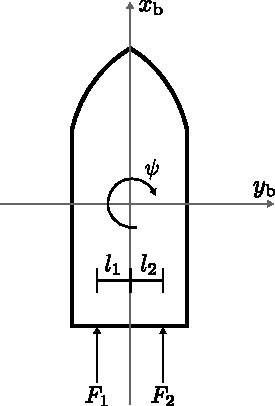
\includegraphics[width=0.7\linewidth]{figures/boat2D}
        \end{figure}                
    \end{minipage}\hfill \\
\end{frame}

%\subsection{Model Equations}
\begin{frame}{Model}{Model Equations}
    \begin{flalign}
        m \ddot{x}_\mathrm{b} &=  F_\mathrm{1} + F_\mathrm{2}  - d_{\dot{x}_\mathrm{b}} \dot{x}_\mathrm{b} + F_{x_\mathrm{b}}  \nonumber \\
        m \ddot{y}_\mathrm{b} &=  -d_{\dot{y}_\mathrm{b}} \dot{y_\mathrm{b}} + F_{y_\mathrm{b}}  \nonumber \\
        m \ddot{z}_\mathrm{b} &=  -d_{\dot{z}_\mathrm{b}}\dot{z_\mathrm{b}} + F_{z_\mathrm{b}}  \nonumber \\
        I_\mathrm{x}\ddot{\phi} &= -d_{\dot{\phi}} \dot{\phi} + T_\mathrm{\phi}   \nonumber \\
        I_\mathrm{y}\ddot{\theta} &= -d_{\dot{\theta}} \dot{\theta} + T_\mathrm{\theta}   \nonumber \\
        I_\mathrm{z}\ddot{\psi} &= F_\mathrm{1}l_\mathrm{1} - F_\mathrm{2} l_\mathrm{2} - d_{\dot{\psi}} \dot{\psi}  \nonumber
    \end{flalign}
\end{frame}

%\subsection{Model Verification}
\begin{frame}{Model}{Model Verification}
    \begin{minipage}{0.45\linewidth}
        \begin{figure}[H]
            \centering
            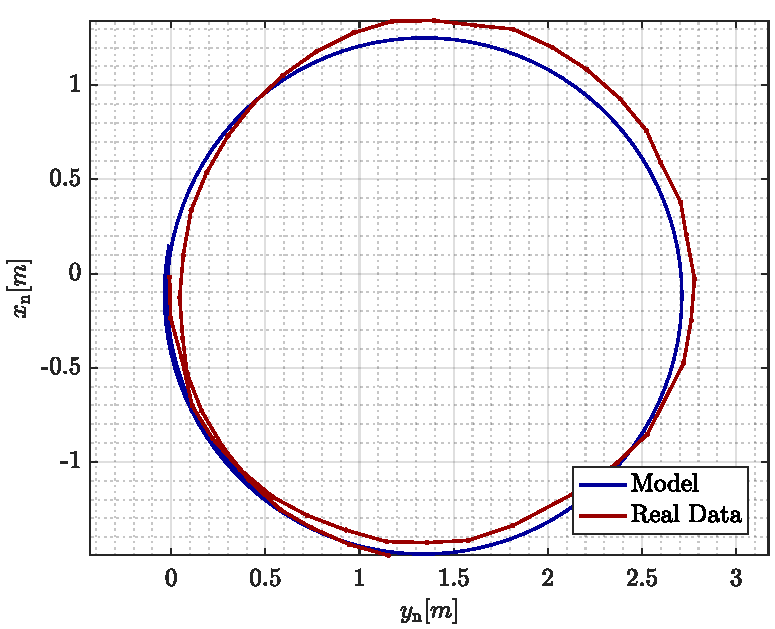
\includegraphics[width=1\linewidth]{figures/turn}
        \end{figure}        
    \end{minipage}\hfill      
    \begin{minipage}{0.45\linewidth}
        \begin{figure}[H]
            \centering
            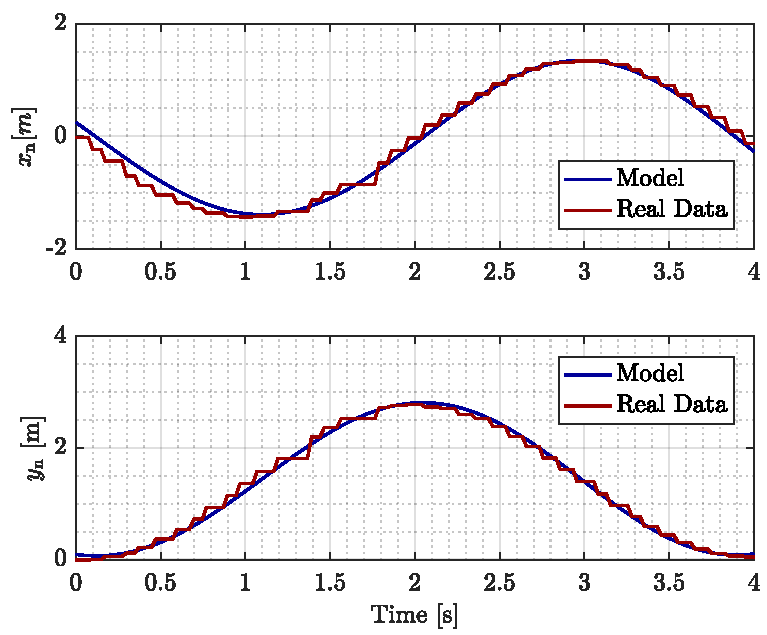
\includegraphics[width=1\linewidth]{figures/turn_time}
        \end{figure}                
    \end{minipage}\hfill \\
\end{frame}






